% generated by Plantuml 1.2023.3       
\definecolor{plantucolor0000}{RGB}{255,255,255}
\definecolor{plantucolor0001}{RGB}{0,0,0}
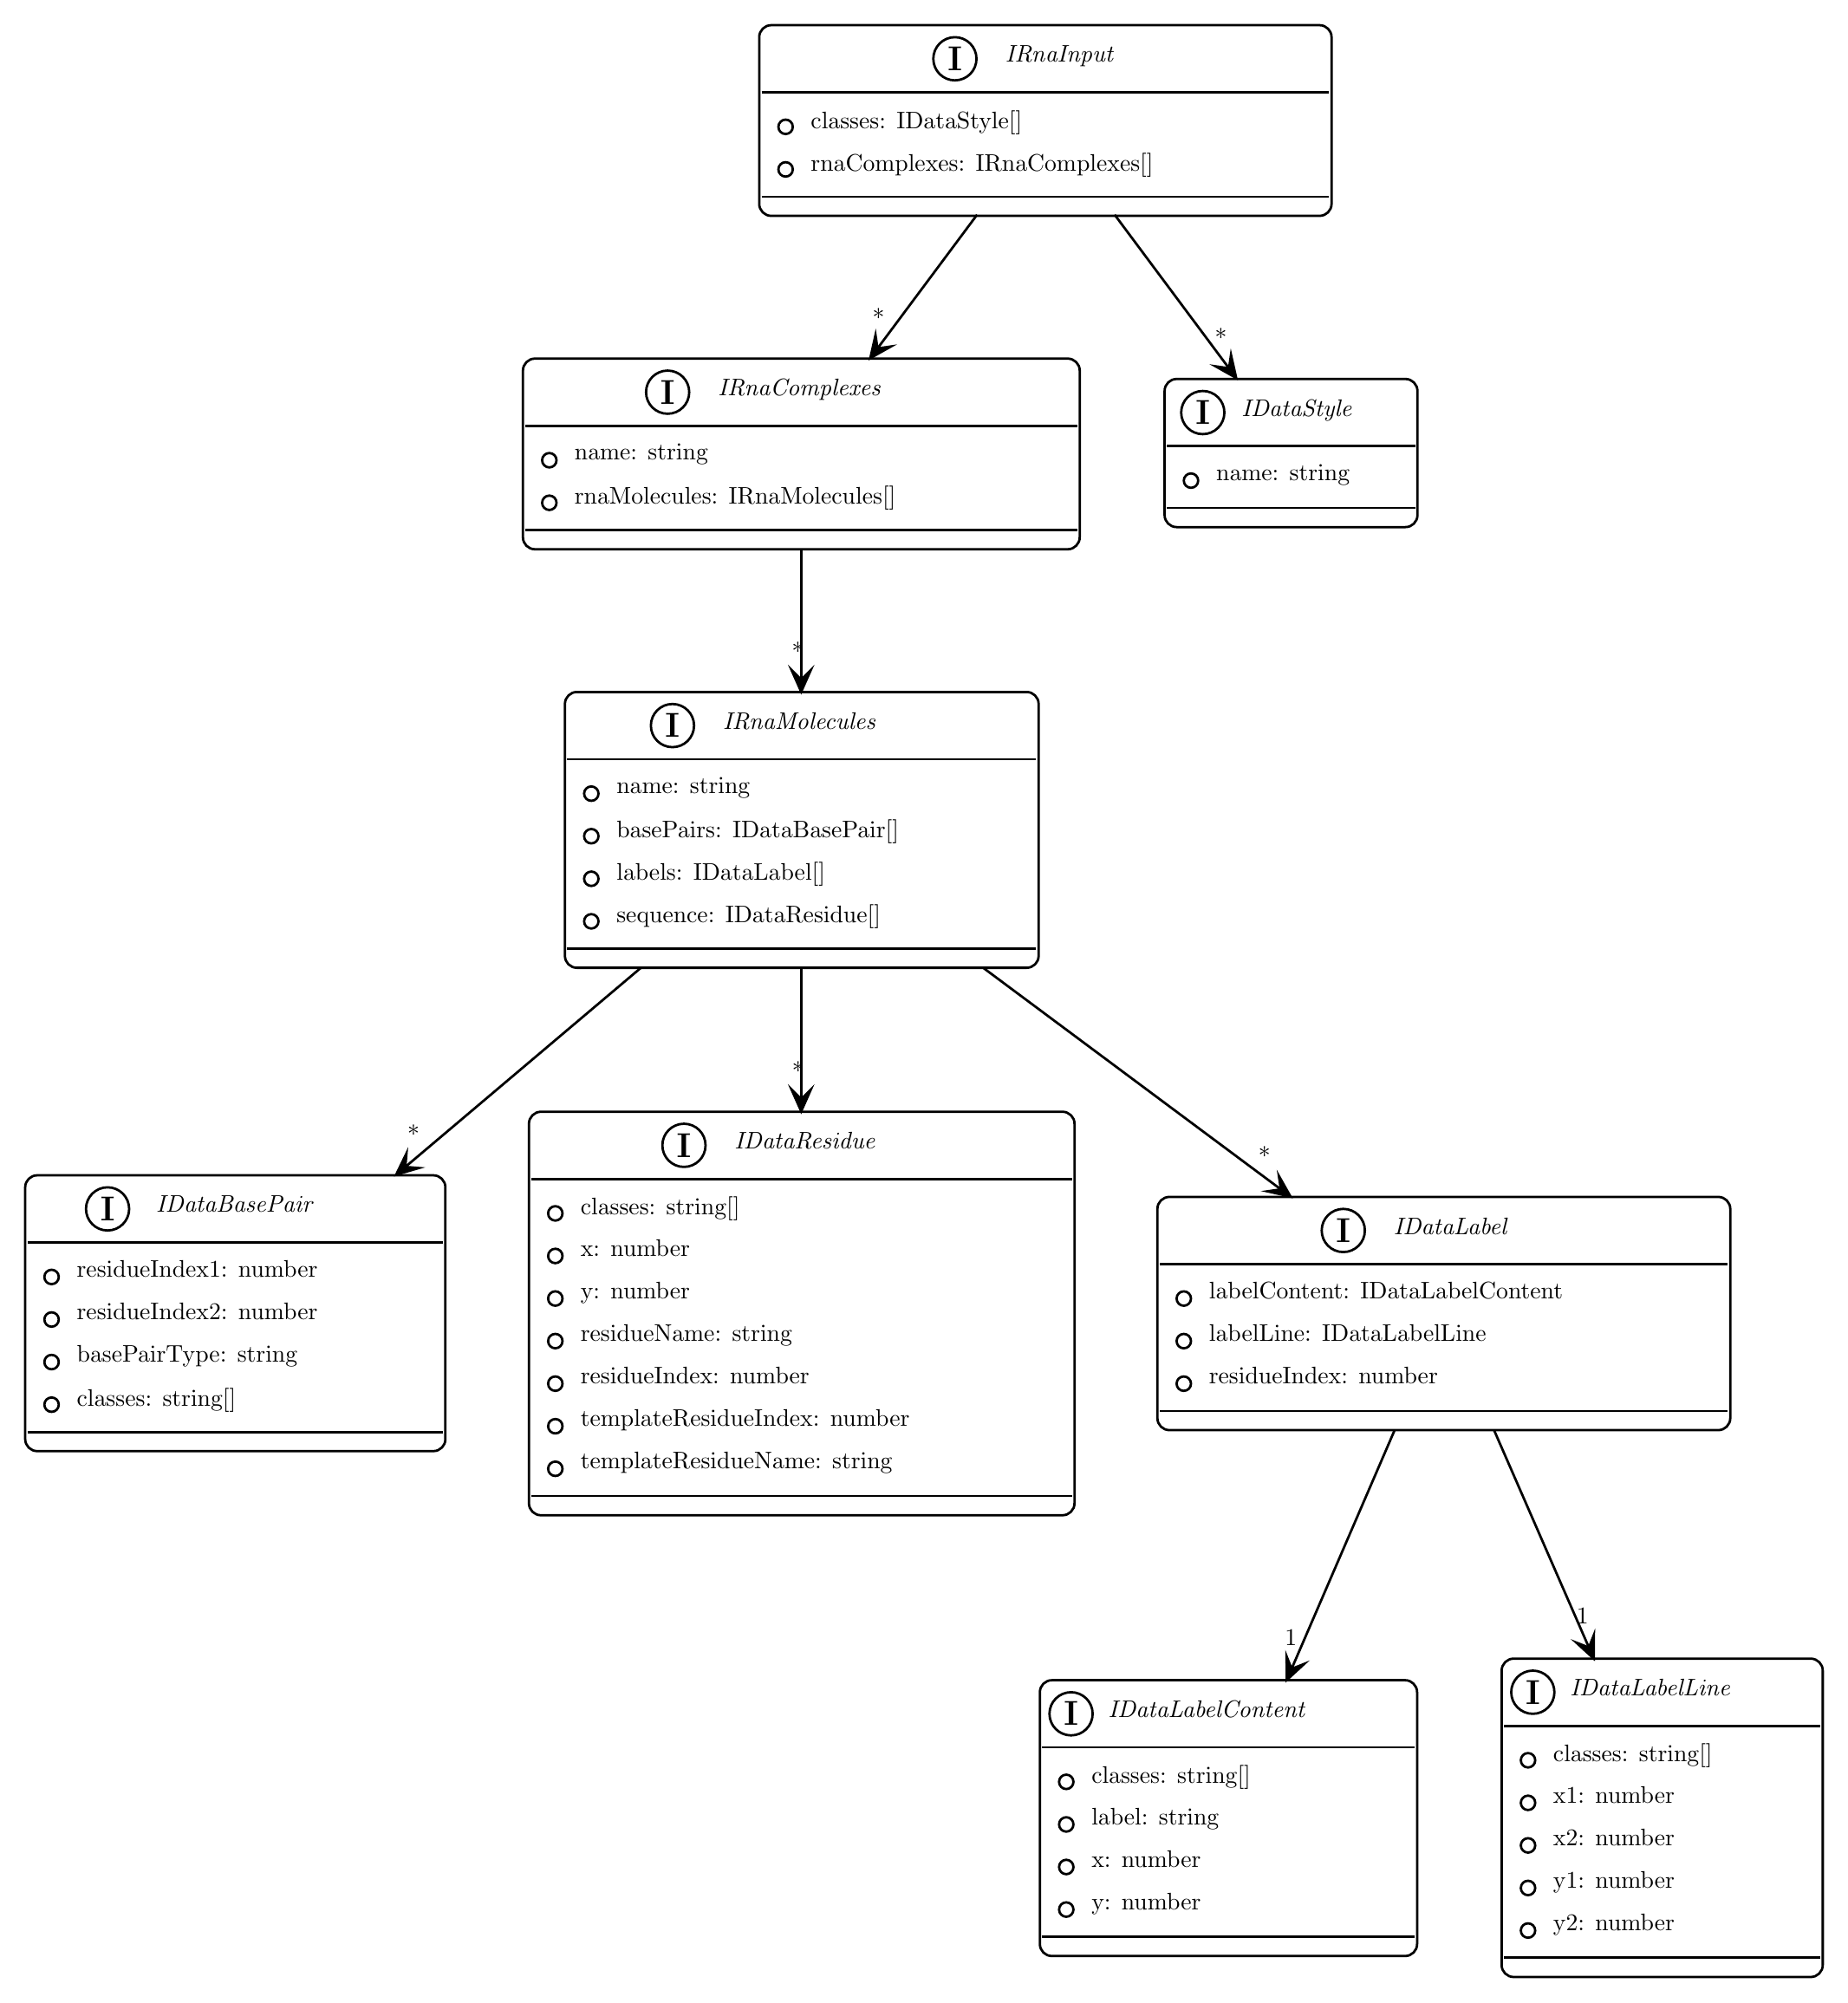
\begin{tikzpicture}[yscale=-1
,pstyle0/.style={color=black,fill=white,line width=1.0pt}
,pstyle1/.style={color=black,line width=1.0pt}
,pstyle2/.style={color=black,fill=black,line width=1.0pt}
]
\draw[pstyle0] (12pt,496.5pt) arc (180:270:5pt) -- (17pt,491.5pt) -- (182.1721pt,491.5pt) arc (270:360:5pt) -- (187.1721pt,496.5pt) -- (187.1721pt,601.4844pt) arc (0:90:5pt) -- (182.1721pt,606.4844pt) -- (17pt,606.4844pt) arc (90:180:5pt) -- (12pt,601.4844pt) -- cycle;
\draw[pstyle0] (46.3439pt,505.5pt) ellipse (9pt and 9pt);
\node at (46.3439pt,505.5pt)[]{\textbf{\Large I}};
\node at (63.087pt,496.627pt)[below right,color=black]{\textit{IDataBasePair}};
\draw[pstyle1] (13pt,519.5pt) -- (186.1721pt,519.5pt);
\draw[pstyle1] (23pt,533.873pt) ellipse (3pt and 3pt);
\node at (30pt,523.5pt)[below right,color=black]{residueIndex1: number};
\draw[pstyle1] (23pt,551.6191pt) ellipse (3pt and 3pt);
\node at (30pt,541.2461pt)[below right,color=black]{residueIndex2: number};
\draw[pstyle1] (23pt,569.3652pt) ellipse (3pt and 3pt);
\node at (30pt,558.9922pt)[below right,color=black]{basePairType: string};
\draw[pstyle1] (23pt,587.1113pt) ellipse (3pt and 3pt);
\node at (30pt,576.7383pt)[below right,color=black]{classes: string[]};
\draw[pstyle1] (13pt,598.4844pt) -- (186.1721pt,598.4844pt);
\draw[pstyle0] (435pt,707pt) arc (180:270:5pt) -- (440pt,702pt) -- (587.2587pt,702pt) arc (270:360:5pt) -- (592.2587pt,707pt) -- (592.2587pt,811.9844pt) arc (0:90:5pt) -- (587.2587pt,816.9844pt) -- (440pt,816.9844pt) arc (90:180:5pt) -- (435pt,811.9844pt) -- cycle;
\draw[pstyle0] (448pt,716pt) ellipse (9pt and 9pt);
\node at (448pt,716pt)[]{\textbf{\Large I}};
\node at (460pt,707.127pt)[below right,color=black]{\textit{IDataLabelContent}};
\draw[pstyle1] (436pt,730pt) -- (591.2587pt,730pt);
\draw[pstyle1] (446pt,744.373pt) ellipse (3pt and 3pt);
\node at (453pt,734pt)[below right,color=black]{classes: string[]};
\draw[pstyle1] (446pt,762.1191pt) ellipse (3pt and 3pt);
\node at (453pt,751.7461pt)[below right,color=black]{label: string};
\draw[pstyle1] (446pt,779.8652pt) ellipse (3pt and 3pt);
\node at (453pt,769.4922pt)[below right,color=black]{x: number};
\draw[pstyle1] (446pt,797.6113pt) ellipse (3pt and 3pt);
\node at (453pt,787.2383pt)[below right,color=black]{y: number};
\draw[pstyle1] (436pt,808.9844pt) -- (591.2587pt,808.9844pt);
\draw[pstyle0] (627.5pt,698pt) arc (180:270:5pt) -- (632.5pt,693pt) -- (756.3667pt,693pt) arc (270:360:5pt) -- (761.3667pt,698pt) -- (761.3667pt,820.7305pt) arc (0:90:5pt) -- (756.3667pt,825.7305pt) -- (632.5pt,825.7305pt) arc (90:180:5pt) -- (627.5pt,820.7305pt) -- cycle;
\draw[pstyle0] (640.5pt,707pt) ellipse (9pt and 9pt);
\node at (640.5pt,707pt)[]{\textbf{\Large I}};
\node at (652.5pt,698.127pt)[below right,color=black]{\textit{IDataLabelLine}};
\draw[pstyle1] (628.5pt,721pt) -- (760.3667pt,721pt);
\draw[pstyle1] (638.5pt,735.373pt) ellipse (3pt and 3pt);
\node at (645.5pt,725pt)[below right,color=black]{classes: string[]};
\draw[pstyle1] (638.5pt,753.1191pt) ellipse (3pt and 3pt);
\node at (645.5pt,742.7461pt)[below right,color=black]{x1: number};
\draw[pstyle1] (638.5pt,770.8652pt) ellipse (3pt and 3pt);
\node at (645.5pt,760.4922pt)[below right,color=black]{x2: number};
\draw[pstyle1] (638.5pt,788.6113pt) ellipse (3pt and 3pt);
\node at (645.5pt,778.2383pt)[below right,color=black]{y1: number};
\draw[pstyle1] (638.5pt,806.3574pt) ellipse (3pt and 3pt);
\node at (645.5pt,795.9844pt)[below right,color=black]{y2: number};
\draw[pstyle1] (628.5pt,817.7305pt) -- (760.3667pt,817.7305pt);
\draw[pstyle0] (222pt,470pt) arc (180:270:5pt) -- (227pt,465pt) -- (444.4382pt,465pt) arc (270:360:5pt) -- (449.4382pt,470pt) -- (449.4382pt,628.2227pt) arc (0:90:5pt) -- (444.4382pt,633.2227pt) -- (227pt,633.2227pt) arc (90:180:5pt) -- (222pt,628.2227pt) -- cycle;
\draw[pstyle0] (286.6262pt,479pt) ellipse (9pt and 9pt);
\node at (286.6262pt,479pt)[]{\textbf{\Large I}};
\node at (304.1262pt,470.127pt)[below right,color=black]{\textit{IDataResidue}};
\draw[pstyle1] (223pt,493pt) -- (448.4382pt,493pt);
\draw[pstyle1] (233pt,507.373pt) ellipse (3pt and 3pt);
\node at (240pt,497pt)[below right,color=black]{classes: string[]};
\draw[pstyle1] (233pt,525.1191pt) ellipse (3pt and 3pt);
\node at (240pt,514.7461pt)[below right,color=black]{x: number};
\draw[pstyle1] (233pt,542.8652pt) ellipse (3pt and 3pt);
\node at (240pt,532.4922pt)[below right,color=black]{y: number};
\draw[pstyle1] (233pt,560.6113pt) ellipse (3pt and 3pt);
\node at (240pt,550.2383pt)[below right,color=black]{residueName: string};
\draw[pstyle1] (233pt,578.3574pt) ellipse (3pt and 3pt);
\node at (240pt,567.9844pt)[below right,color=black]{residueIndex: number};
\draw[pstyle1] (233pt,596.1035pt) ellipse (3pt and 3pt);
\node at (240pt,585.7305pt)[below right,color=black]{templateResidueIndex: number};
\draw[pstyle1] (233pt,613.8496pt) ellipse (3pt and 3pt);
\node at (240pt,603.4766pt)[below right,color=black]{templateResidueName: string};
\draw[pstyle1] (223pt,625.2227pt) -- (448.4382pt,625.2227pt);
\draw[pstyle0] (219.5pt,156pt) arc (180:270:5pt) -- (224.5pt,151pt) -- (446.6091pt,151pt) arc (270:360:5pt) -- (451.6091pt,156pt) -- (451.6091pt,225.4922pt) arc (0:90:5pt) -- (446.6091pt,230.4922pt) -- (224.5pt,230.4922pt) arc (90:180:5pt) -- (219.5pt,225.4922pt) -- cycle;
\draw[pstyle0] (279.8227pt,165pt) ellipse (9pt and 9pt);
\node at (279.8227pt,165pt)[]{\textbf{\Large I}};
\node at (297.3227pt,156.127pt)[below right,color=black]{\textit{IRnaComplexes}};
\draw[pstyle1] (220.5pt,179pt) -- (450.6091pt,179pt);
\draw[pstyle1] (230.5pt,193.373pt) ellipse (3pt and 3pt);
\node at (237.5pt,183pt)[below right,color=black]{name: string};
\draw[pstyle1] (230.5pt,211.1191pt) ellipse (3pt and 3pt);
\node at (237.5pt,200.7461pt)[below right,color=black]{rnaMolecules: IRnaMolecules[]};
\draw[pstyle1] (220.5pt,222.4922pt) -- (450.6091pt,222.4922pt);
\draw[pstyle0] (237pt,295pt) arc (180:270:5pt) -- (242pt,290pt) -- (429.4846pt,290pt) arc (270:360:5pt) -- (434.4846pt,295pt) -- (434.4846pt,399.9844pt) arc (0:90:5pt) -- (429.4846pt,404.9844pt) -- (242pt,404.9844pt) arc (90:180:5pt) -- (237pt,399.9844pt) -- cycle;
\draw[pstyle0] (281.8393pt,304pt) ellipse (9pt and 9pt);
\node at (281.8393pt,304pt)[]{\textbf{\Large I}};
\node at (299.3393pt,295.127pt)[below right,color=black]{\textit{IRnaMolecules}};
\draw[pstyle1] (238pt,318pt) -- (433.4846pt,318pt);
\draw[pstyle1] (248pt,332.373pt) ellipse (3pt and 3pt);
\node at (255pt,322pt)[below right,color=black]{name: string};
\draw[pstyle1] (248pt,350.1191pt) ellipse (3pt and 3pt);
\node at (255pt,339.7461pt)[below right,color=black]{basePairs: IDataBasePair[]};
\draw[pstyle1] (248pt,367.8652pt) ellipse (3pt and 3pt);
\node at (255pt,357.4922pt)[below right,color=black]{labels: IDataLabel[]};
\draw[pstyle1] (248pt,385.6113pt) ellipse (3pt and 3pt);
\node at (255pt,375.2383pt)[below right,color=black]{sequence: IDataResidue[]};
\draw[pstyle1] (238pt,396.9844pt) -- (433.4846pt,396.9844pt);
\draw[pstyle0] (318pt,17pt) arc (180:270:5pt) -- (323pt,12pt) -- (551.5978pt,12pt) arc (270:360:5pt) -- (556.5978pt,17pt) -- (556.5978pt,86.4922pt) arc (0:90:5pt) -- (551.5978pt,91.4922pt) -- (323pt,91.4922pt) arc (90:180:5pt) -- (318pt,86.4922pt) -- cycle;
\draw[pstyle0] (399.5765pt,26pt) ellipse (9pt and 9pt);
\node at (399.5765pt,26pt)[]{\textbf{\Large I}};
\node at (417.0765pt,17.127pt)[below right,color=black]{\textit{IRnaInput}};
\draw[pstyle1] (319pt,40pt) -- (555.5978pt,40pt);
\draw[pstyle1] (329pt,54.373pt) ellipse (3pt and 3pt);
\node at (336pt,44pt)[below right,color=black]{classes: IDataStyle[]};
\draw[pstyle1] (329pt,72.1191pt) ellipse (3pt and 3pt);
\node at (336pt,61.7461pt)[below right,color=black]{rnaComplexes: IRnaComplexes[]};
\draw[pstyle1] (319pt,83.4922pt) -- (555.5978pt,83.4922pt);
\draw[pstyle0] (487pt,164.5pt) arc (180:270:5pt) -- (492pt,159.5pt) -- (587.4087pt,159.5pt) arc (270:360:5pt) -- (592.4087pt,164.5pt) -- (592.4087pt,216.2461pt) arc (0:90:5pt) -- (587.4087pt,221.2461pt) -- (492pt,221.2461pt) arc (90:180:5pt) -- (487pt,216.2461pt) -- cycle;
\draw[pstyle0] (502.9139pt,173.5pt) ellipse (9pt and 9pt);
\node at (502.9139pt,173.5pt)[]{\textbf{\Large I}};
\node at (515.5614pt,164.627pt)[below right,color=black]{\textit{IDataStyle}};
\draw[pstyle1] (488pt,187.5pt) -- (591.4087pt,187.5pt);
\draw[pstyle1] (498pt,201.873pt) ellipse (3pt and 3pt);
\node at (505pt,191.5pt)[below right,color=black]{name: string};
\draw[pstyle1] (488pt,213.2461pt) -- (591.4087pt,213.2461pt);
\draw[pstyle0] (484pt,505.5pt) arc (180:270:5pt) -- (489pt,500.5pt) -- (717.8133pt,500.5pt) arc (270:360:5pt) -- (722.8133pt,505.5pt) -- (722.8133pt,592.7383pt) arc (0:90:5pt) -- (717.8133pt,597.7383pt) -- (489pt,597.7383pt) arc (90:180:5pt) -- (484pt,592.7383pt) -- cycle;
\draw[pstyle0] (561.4874pt,514.5pt) ellipse (9pt and 9pt);
\node at (561.4874pt,514.5pt)[]{\textbf{\Large I}};
\node at (578.9874pt,505.627pt)[below right,color=black]{\textit{IDataLabel}};
\draw[pstyle1] (485pt,528.5pt) -- (721.8133pt,528.5pt);
\draw[pstyle1] (495pt,542.873pt) ellipse (3pt and 3pt);
\node at (502pt,532.5pt)[below right,color=black]{labelContent: IDataLabelContent};
\draw[pstyle1] (495pt,560.6191pt) ellipse (3pt and 3pt);
\node at (502pt,550.2461pt)[below right,color=black]{labelLine: IDataLabelLine};
\draw[pstyle1] (495pt,578.3652pt) ellipse (3pt and 3pt);
\node at (502pt,567.9922pt)[below right,color=black]{residueIndex: number};
\draw[pstyle1] (485pt,589.7383pt) -- (721.8133pt,589.7383pt);
\draw[pstyle1] (335.5pt,230.21pt) ..controls (335.5pt,246.69pt) and (335.5pt,266.31pt) .. (335.5pt,284.71pt);
\draw[pstyle2] (335.5pt,289.86pt) -- (339.5pt,280.86pt) -- (335.5pt,284.86pt) -- (331.5pt,280.86pt) -- (335.5pt,289.86pt) -- cycle;
\node at (328.0736pt,265.4815pt)[below right,color=black]{*};
\draw[pstyle1] (268.5pt,405.14pt) ..controls (237.99pt,430.93pt) and (201.83pt,461.5pt) .. (170.81pt,487.72pt);
\draw[pstyle2] (166.66pt,491.22pt) -- (176.1138pt,488.4585pt) -- (170.4764pt,487.9896pt) -- (170.9452pt,482.3523pt) -- (166.66pt,491.22pt) -- cycle;
\node at (167.8585pt,466.8236pt)[below right,color=black]{*};
\draw[pstyle1] (411.58pt,405.14pt) ..controls (450.55pt,434.14pt) and (497.61pt,469.18pt) .. (535.38pt,497.29pt);
\draw[pstyle2] (539.47pt,500.34pt) -- (534.6357pt,491.7593pt) -- (535.458pt,497.356pt) -- (529.8613pt,498.1784pt) -- (539.47pt,500.34pt) -- cycle;
\node at (522.6261pt,476.0357pt)[below right,color=black]{*};
\draw[pstyle1] (335.5pt,405.14pt) ..controls (335.5pt,422.09pt) and (335.5pt,441.1pt) .. (335.5pt,459.58pt);
\draw[pstyle2] (335.5pt,464.78pt) -- (339.5pt,455.78pt) -- (335.5pt,459.78pt) -- (331.5pt,455.78pt) -- (335.5pt,464.78pt) -- cycle;
\node at (328.2057pt,440.578pt)[below right,color=black]{*};
\draw[pstyle1] (466.18pt,91.03pt) ..controls (481.08pt,111.04pt) and (499.15pt,135.31pt) .. (513.62pt,154.74pt);
\draw[pstyle2] (516.84pt,159.06pt) -- (514.6784pt,149.4513pt) -- (513.856pt,155.048pt) -- (508.2593pt,154.2257pt) -- (516.84pt,159.06pt) -- cycle;
\node at (504.4878pt,135.001pt)[below right,color=black]{*};
\draw[pstyle1] (408.82pt,91.03pt) ..controls (396pt,108.25pt) and (380.83pt,128.61pt) .. (367.63pt,146.34pt);
\draw[pstyle2] (364.32pt,150.79pt) -- (372.9007pt,145.9557pt) -- (367.304pt,146.778pt) -- (366.4816pt,141.1813pt) -- (364.32pt,150.79pt) -- cycle;
\node at (361.7337pt,126.5887pt)[below right,color=black]{*};
\draw[pstyle1] (582.96pt,597.57pt) ..controls (570.21pt,627.13pt) and (553.68pt,665.42pt) .. (539.95pt,697.23pt);
\draw[pstyle2] (537.94pt,701.87pt) -- (545.1869pt,695.2005pt) -- (539.9268pt,697.2817pt) -- (537.8457pt,692.0216pt) -- (537.94pt,701.87pt) -- cycle;
\node at (533.6192pt,677.4928pt)[below right,color=black]{1};
\draw[pstyle1] (624.26pt,597.57pt) ..controls (635.96pt,624.38pt) and (650.8pt,658.38pt) .. (663.82pt,688.21pt);
\draw[pstyle2] (665.89pt,692.96pt) -- (665.9585pt,683.1114pt) -- (663.8912pt,688.3769pt) -- (658.6256pt,686.3095pt) -- (665.89pt,692.96pt) -- cycle;
\node at (655.1966pt,668.3846pt)[below right,color=black]{1};
\end{tikzpicture}
